\chapter{Data Analysis}
\label{sec:data_analysis}
\label{sec:eda}

This chapter presents exploratory data analysis of the Styrian Health Data at the individual level, covering data preparation, descriptive patterns, and group comparisons that inform the modelling in Chapter~\ref{sec:modelling}.

\section{Data Preparation and Quality Assessment}
\label{sec:eda_prep}

The raw dataset contains 16,386 records with heterogeneous missing values. After removing incomplete and implausible entries and restricting ages to the range 13--100 years, a final analysis sample of 15,219 observations remains (7.1\% excluded).

Key data quality characteristics are summarised below:
\begin{itemize}
    \item 23 records are missing all core demographic and health variables (\texttt{befinden}, birth year, gender, and age).
    \item Column-wise missingness includes 331 missing state identifiers and 45--56 missing blood pressure estimates.
    \item Temporal coverage spans April to October 2006, with 373 measurements recorded before 10:00 and 116 after 18:00.
    \item Geographic coverage is concentrated in Styria, accounting for approximately 89\% of records with valid state information.
\end{itemize}

Mean imputation for missing values was considered but not applied, as it was deemed likely to introduce bias into subsequent analyses.

\section{Demographics and Health Status}
\label{sec:eda_demographics}

Self-reported health status (\texttt{befinden}, scale 1--5) is heavily concentrated in the lower categories, as shown in Table~\ref{tab:level_counts}.

\begin{table}[h]
    \centering
    \caption{Distribution of self-reported health status (\texttt{befinden}).}
    \label{tab:level_counts}
    \begin{tabular}{cc}
        \toprule
        \textbf{Health Level} & \textbf{Count} \\
        \midrule
        1 & 5,897 \\
        2 & 7,931 \\
        3 & 2,240 \\
        4 & 198 \\
        5 & 97 \\
        \bottomrule
    \end{tabular}
\end{table}

The correlation structure of the numerical variables indicates generally weak to moderate linear relationships, visualised in Figure~\ref{fig:heatmap}. The strongest correlation is observed between systolic and diastolic measured blood pressure ($r \approx 0.67$), while estimated and measured blood pressure values also show moderate association. Age exhibits only weak correlations with other variables, and health status shows minimal linear association with the remaining features.

\begin{figure}[h]
    \centering
    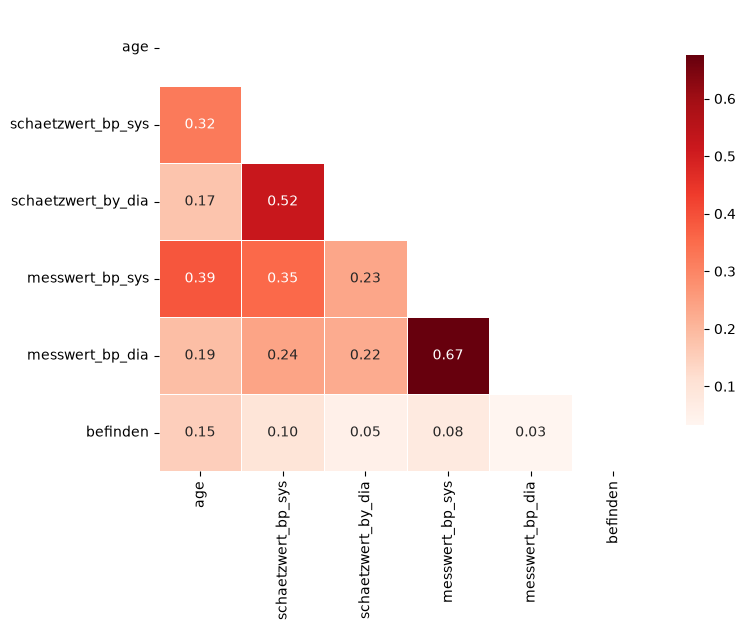
\includegraphics[width=0.75\textwidth]{figures/heatmap_lowertri.png}
    \caption{Lower-triangular correlation heatmap of selected numerical variables. Darker shading indicates stronger positive or negative Pearson correlation.}
    \label{fig:heatmap}
\end{figure}

Missing values were not fully random. Records with missing self-reported health condition often had missing values in other fields as well, indicating incomplete participant records rather than isolated recording errors. Most participants were between 30 and 70 years old; Figure~\ref{fig:age_dist} shows that the age distribution reflects a predominantly adult sample, which is appropriate for studying blood pressure variation.

The data also contain implausible entries. For example, there are 11 smokers below the age of 5 and birth years extending as far back as 1880, which likely indicate data entry errors rather than genuine observations.

\begin{figure}[h]
    \centering
    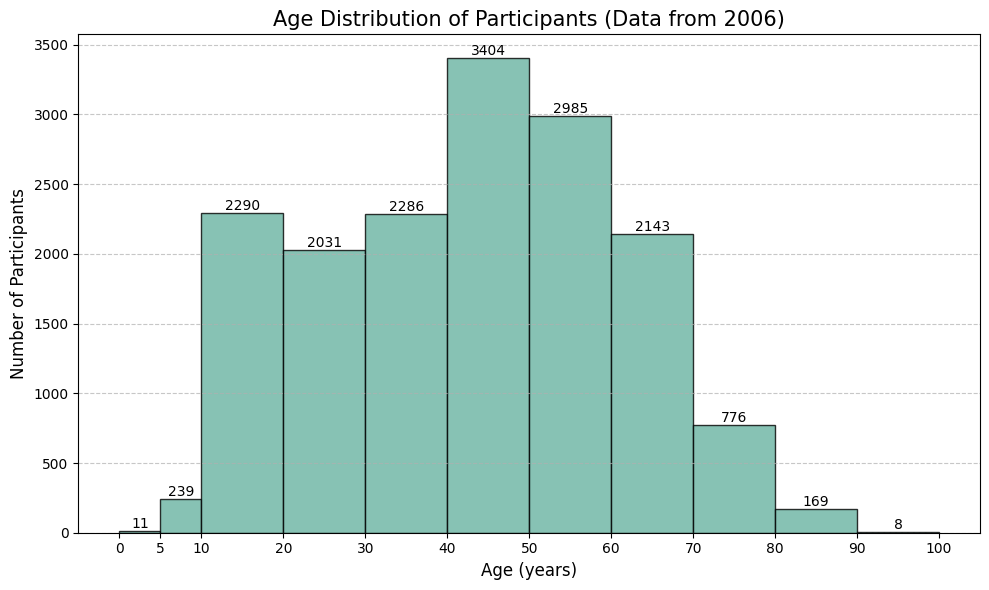
\includegraphics[width=0.6\textwidth]{figures/age_dist.png}
    \caption{Age distribution of participants in the analysis sample ($n = 15{,}219$).}
    \label{fig:age_dist}
\end{figure}

\section{Measured and Self-Estimated Blood Pressure}
\label{sec:eda_bp}

Figure~\ref{fig:bp_comparison} compares the distributional shapes of measured and self-estimated blood pressure. Density is defined such that the area under each curve equals one, allowing a comparison of shapes independent of sample size differences across groups.

\begin{figure}[h]
    \centering
    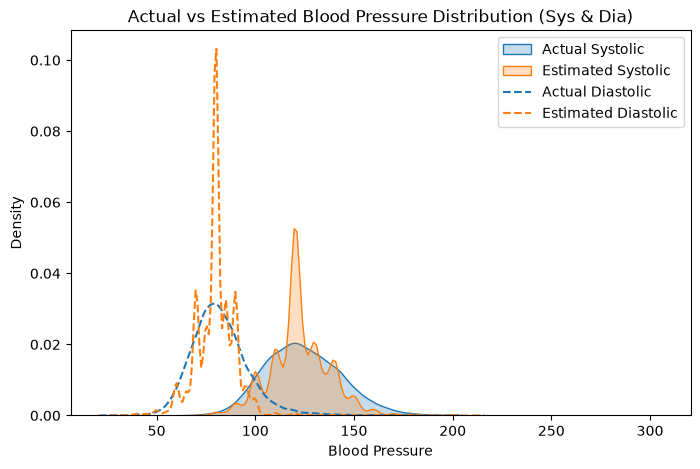
\includegraphics[width=0.7\textwidth]{figures/act_estimated_bp.png}
    \caption{Kernel density estimates of measured and self-estimated systolic and diastolic blood pressure.}
    \label{fig:bp_comparison}
\end{figure}

The distribution of measured blood pressure is notably more dispersed than that of self-estimated values, particularly for systolic pressure. This suggests that participants tend to report values clustered around common or rounded reference points, whereas the measured data exhibit substantially greater variability.

\section{Group Differences and Correlations}
\label{sec:eda_groups}

Figure~\ref{fig:gender_comparison} shows that male participants exhibit higher average systolic and diastolic blood pressure compared to female participants, although both groups display considerable internal variability.

\begin{figure}[h]
    \centering
    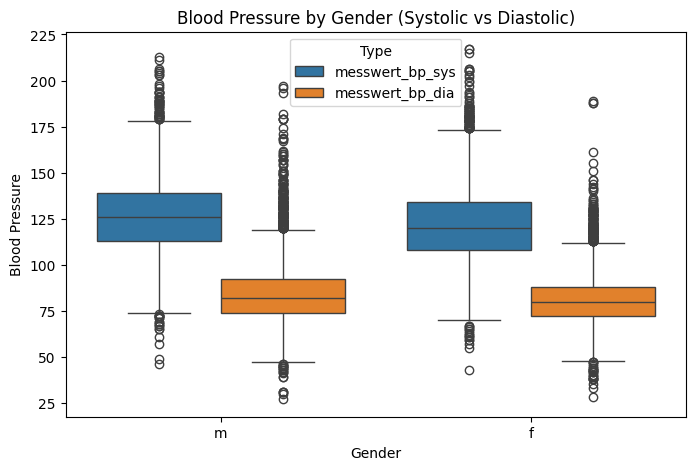
\includegraphics[width=0.7\textwidth]{figures/gender_comparison.png}
    \caption{Blood pressure and self-reported health status by gender. Box plots summarise the central tendency and spread within each group.}
    \label{fig:gender_comparison}
\end{figure}

The correlation analysis indicates a strong positive association between measured systolic and diastolic blood pressure. Age shows a moderate correlation with both outcomes. Self-estimated blood pressure values are also positively correlated with measured values; however, these relationships are weaker than the correlation observed between the two measured blood pressure variables.

\section{Risk Factor Comparisons}
\label{sec:eda_risk}

Group comparisons confirm several statistically significant differences, summarised in Table~\ref{tab:risk_factors}.

\begin{table}[h]
    \centering
    \caption{Mean blood pressure differences across risk groups. Values are group means in mmHg; \textit{p} denotes the two-sample test significance level.}
    \label{tab:risk_factors}
    \begin{tabular}{llcc}
        \toprule
        \textbf{Comparison} & \textbf{Systolic} & \textbf{Diastolic} \\
        \midrule
        Male vs.\ Female & 128.0 vs.\ 122.8 ($p<0.001$) & 84.6 vs.\ 81.0 ($p<0.001$) \\
        Smoker vs.\ Non-smoker & 122.9 vs.\ 125.5 ($p<0.001$) & 82.5 vs.\ 82.6 (not significant) \\
        Blood sugar known vs.\ not & 128.8 vs.\ 123.7 ($p<0.001$) & 83.8 vs.\ 82.1 ($p<0.001$) \\
        Cholesterol known vs.\ not & 128.0 vs.\ 123.4 ($p<0.001$) & 83.5 vs.\ 82.0 ($p<0.001$) \\
        In treatment vs.\ not & 137.8 vs.\ 123.2 ($p<0.001$) & 86.4 vs.\ 82.0 ($p<0.001$) \\
        \bottomrule
    \end{tabular}
\end{table}

Higher blood pressure among individuals with known conditions likely reflects confounding due to increased medical awareness and pre-existing health conditions rather than a direct causal effect of the awareness indicator itself.
